\chapter{Desarrollo del Detector de Rostros y la Arquitectura de Red Neuronal Convolucional}

\section{Detección de Rostros}
En este trabajo se optó por utilizar como etapa inicial dentro de la fase de consultas a la red, la construcción de un detector de rostros, debido a que, al momento de desarrollar una aplicación orientada a las necesidades del mundo real, este no solo recibira como entrada imágenes que contengan exactamente el rostro de la persona, sino, imágenes con el cuerpo completo o algunas partes adicionales aparte del rostro. Sin embargo, en objetivo del trabajo es poder detectar la expresión facial de una persona, para lo cual, basta con tener como entrada a la red una imagen que delimite el rostro de la persona. De ahí, la necesidad de utilizar un algoritmo de detección de rostros para la extracción de la región de interes que posteriormente servira como entrada para la red neuronal convolucional encargada de reconocer la expresión facial correspondiente. La figura~\ref{fig:imagen_entrada} muestra un ejemplo de una imagen de entrada, en la cual, se puede observar detalles adicionales aparte del rostro(el sombrero y el fondo), los cuales no aportan carasteristicas relevantes que ayuden al reconocimiento de la expresion facial.

Para esta etapa se utilizó el detector de objetos \textit{Haar Cascade}, un algoritmo muy utilizado, cuya implementación puede ser encontrado en distintas librerías orientadas al procesamiento de imágenes, tales como OpenCV\footnote[5]{OpenCV es una librería \textit{open source} que contiene algoritmo relacionados con el area de visión por computador, http://opencv.org/}. Como se describió en la sección~\ref{sec:Haar_Cascade}, este algoritmo utiliza técnicas de \textit{machine learning}. Su proceso de entrenamiento se realiza con imágenes positivas y negativas(imágenes que representan y no representan rostros), creando así un modelo capaz de detectar rostros, basandose en la detecciín de caracteristicas \textit{Haar}. La entrada para esta etapa es una imagen cualquiera, el proceso consiste en detectar el rostro en dicha imagen(en caso exista algun rostro) y extraerlo en otra imagen en escala de grises, la cual tendra un tamaño aproximado de 48x48 pixeles(dependiendo de las dimensiones del rostro). Esta última imagen será la entrada para el modelo en la fase de consultas. Nótese que para la detección de un rostro y la asignación de su respectiva expresión facial, no es necesario mantener la imagen a coloros, puesto que este no es una característica necesaria para conseguir el objetivo. La figura~\ref{fig:proceso_deteccion} muestra los pasos a seguir para la detección y extracción del rostro en una imagen.

\begin{figure}[H]
		\centering
		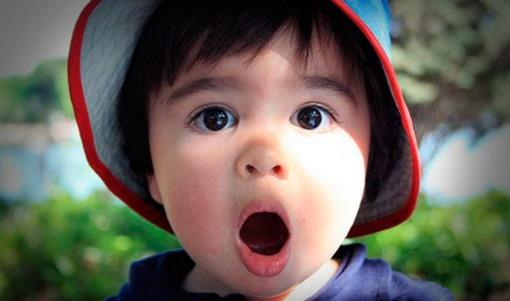
\includegraphics[width=50mm]{./Imagenes/imagen_entrada.png}
		\caption{Ejemplo de una imagen de entrada.}
		\vspace{0.15cm}
		\textit{Fuente: Consuelo Ferrús, http://www.acompasando.org/orar-el-asombro/}
		\label{fig:imagen_entrada}
\end{figure}


\begin{figure}[H]
		\centering
		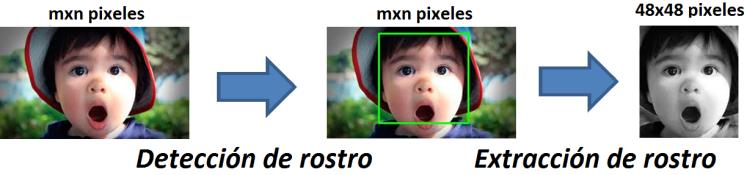
\includegraphics[width=140mm]{./Imagenes/proceso_deteccion.png}
		\caption{Proceso de detección de rostro.}
		\vspace{0.15cm}
		\textit{Fuente: Propio}
		\label{fig:proceso_deteccion}
\end{figure}

Se optó por la utilización del detector de rostros \textit{Haar Cascade}, debido a que este es ampliamente utilizado por el nivel de precisión que posee~\cite{6russakovsky2015imagenet}. Sin embargo, esta técnica aun presenta algunas fallas cuando el rostro presenta algún tipo de oclusión(figura~\ref{fig:oclussion}). Este tipo de problema tambien puede ser solucionado construyendo una red convolucional orientada a la detección o localización de rostros, o por medio de otro tipo de técnicas tradicionales basadas en la extracción de características. Debido al tiempo y bajos recursos computacionales, se opto por proponer este tipo de enfoques como trabajos futuros.

\begin{figure}[H]
		\centering
		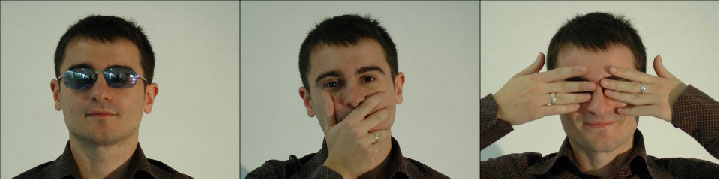
\includegraphics[width=130mm]{./Imagenes/oclussion.jpeg}
		\caption{Ejemplo de rostros con oclusión.}
		\vspace{0.15cm}
		\textit{Fuente: Face Dataset, Universidad Politécnica de Catalunya.}
		\label{fig:oclussion}
\end{figure}

\section{Experimentación en la Elección de Parámetros y Capas en la Construcción de la Arquitectura CNN}
\label{sec:experiment}
La creación de un modelo robusto a partir de la utilización de redes neuronales convolucionales, es una tarea muy complicada, debido a que en la actualidad no existen estudios que indique cual es la configuración correcta que esta debe seguir. Es así, que todos los trabajos que utilizan cualquier técnica perteneciente a \textit{deep learning}, se basan en la experimentación sobre diversar configuraciones en la arquitectura, estas configuraciones estan relacionadas con el numero de capas de convolución, sub-muestreo, totalmente conectadas, tipos de funciones de activacion y normalizacion. Otros elementos muy importantes que tambien son considerados al momento de realizar experimentos, son los parámetros de cada capa, tales como: el número y tamaño de los filtros en la capa de convolucion, operaciones de agrupación en la capa de sub-muestreo, etc.

Sin embargo, entrenar un red neuronal no es una tarea fácil, debido a que se tienen que optimizar miles de parametros para la creación de un buen modelo, asi como las miles de multiplicaciones de matrices que tienen que llevarse a cabo para realizar la operación de convolución. Es así que el número de experimentos que se puedan realizar, depende mucho de la insfraestructura y \textit{hardware} sobre el cual se esta trabajando, siendo este una gran limitante para una extensa experimentación.

Según lo explicado en los parrafos anteriores, para encontrar la correcta configuracion de una arquitectura basada en las redes neuronales convolucionales que resuelva el problema de reconocimiento de expresiones faciales, se realizaron muchos experimentos, cada uno con una configuracion diferente que la anterior. En total se evaluaron 3 arquitecturas con distintas configuracion de capas y parametros, en cada una de estas se calculo la precision y error utilizando las bases de datos FER2013 y CK.




\begin{itemize}
\item {\textbf{Conv-Conv-Pool-Conv-Conv-Pool-FC}

\begin{table}[H]
    \centering
    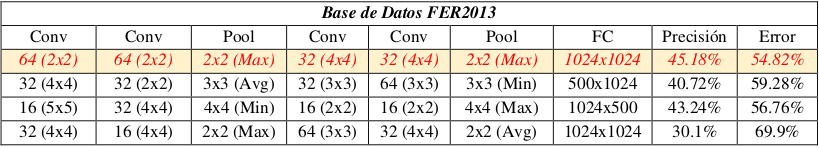
\includegraphics[width=140mm]{./Imagenes/tabla_arqui_1_fer.png} 
    \caption{Evaluación de la arquitectura 1 y sus parámetros, FER2013}
    \label{tab:tabla_arqui_1_fer}
\end{table}

\begin{table}[H]
    \centering
    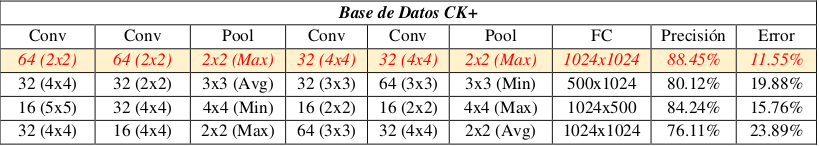
\includegraphics[width=140mm]{./Imagenes/tabla_arqui_1_CK.png}
    \caption{Evaluación de la arquitectura 1 y sus parámetros, CK+}
    \label{tab:tabla_arqui_1_CK}
\end{table}

}

\item {\textbf{Conv-Pool-Conv-Pool-FC \underline{\textit{Arquitectura Propuesta}} }

\begin{table}[H]
    \centering
    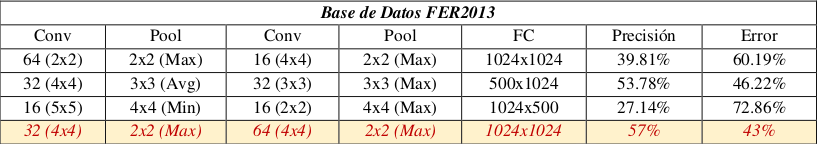
\includegraphics[width=140mm]{./Imagenes/tabla_arqui_2_fer.png} 
    \caption{Evaluación de la arquitectura 2 y sus parámetros, FER2013}
    \label{tab:tabla_arqui_2_fer}
\end{table}

\begin{table}[H]
    \centering
    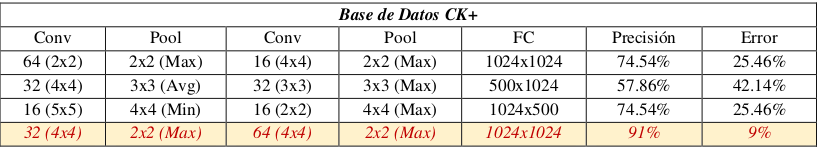
\includegraphics[width=140mm]{./Imagenes/tabla_arqui_2_CK.png}
    \caption{Evaluación de la arquitectura 2 y sus parámetros, CK+}
    \label{tab:tabla_arqui_2_CK}
\end{table}

}

\item {\textbf{Conv-Pool-Pool-Conv-Conv-Pool-FC}

\begin{table}[H]
    \centering
    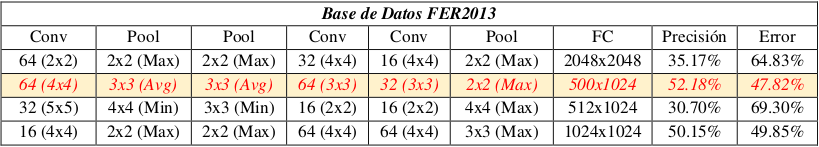
\includegraphics[width=140mm]{./Imagenes/tabla_arqui_3_fer.png} 
    \caption{Evaluación de la arquitectura 3 y sus parámetros, FER2013}
    \label{tab:tabla_arqui_3_fer}
\end{table}

\begin{table}[H]
    \centering
    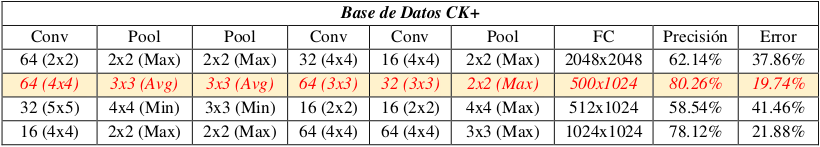
\includegraphics[width=140mm]{./Imagenes/tabla_arqui_3_CK.png}
    \caption{Evaluación de la arquitectura 3 y sus parámetros, CK+}
    \label{tab:tabla_arqui_3_CK}
\end{table}
}
\end{itemize}

De acuerdo con los experimentos realizados, se puede obsevar que la mejor configuracion de capas es: convolucion-\textit{pooling}-convolucion-\textit{pooling}-FC, con 32 y 64 filtros de tamaño 4$\times$4 en la primera y segunda capa de convolucion respectivamente, ventanas de agrupacion de 2$\times$2 en las dos capas de sub-muestreo y un total de 1024$\times$1024 neuronas en las ultimas capas totalmente conectadas.

Segun los resultados mostrados en las tablas~\ref{tab:tabla_arqui_1_fer} y~\ref{tab:tabla_arqui_1_CK} se puede concluir que, la utilización de dos capas consecutivas de convolución es una mala elección, debido a que el hecho de aplicar dos filtros consecutivos hace que la información de la imagen se pierda mas rápidamente que lo normal, ya que el tamaño de la imagen se reduce significativamente después de cada una de estas operaciones. También, las tablas~\ref{tab:tabla_arqui_3_fer} y~\ref{tab:tabla_arqui_3_CK} muestran resultados muy por debajo de la segunda configuración(la mejor obtenida en los experimentos realizados), similar que la explicacion anterior, se concluye que se dan estos resultados debido a la utilizacion de dos capas consecutivas de sub-muestreo, ya que el objetivo de estas capaz es reducir las dimensiones de la imagen solo preservando información reelevante, sin embargo, al realizar una operación de sub-muestreo detras de otra, hace que se pierda mas información de la necesaria. 

\section{Arquitectura Propuesta}
\label{sec:arq_propuesta}
De acuerdo con los experimentados mostrados en la seccion~\ref{sec:experiment}, la arquitectura que consiguio los mejores resultados sigue la siguiente configuracion: la entrada consta de una imagen de 48x48 pixeles en escala de gris, que es el resultado de la fase de detección y extracción de rostro, seguido de una capa de 32 convoluciones con filtro de 4x4 sin solapamiento, luego se aplica un sub muestreo de 2x2 con función MAX \footnote[6]{Función que determina el máximo de n números.} , seguido de una capa de 64 convoluciones con filtros de 2x2 sin solapamiento, para posteriormente aplicar un sub muestreo tambien de dimensiones 2x2 con función MAX, aplicada las convoluciones y sub muestreo se procede a aplicar el Dropout\footnote[7]{Una forma simple de prevenir el \textit{overfitting} en Redes Neuronales..} con 20\%, seguido de dos capas, con 1024 neuronas totalmente conectadas cada una. Finalmente, para la clasificación se aplica la función de normalización Softmax, la cual toma 6 clases, las cuales representar al numero de expresiones a reconocer.
\vspace{0.5cm}
\begin{table}[H]
    \centering
    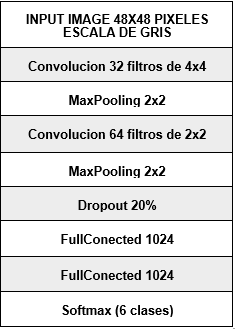
\includegraphics[width=60mm]{./Imagenes/tabla_arquitectura.png}
    \caption{Arquitectura del modelo propuesto}
    \label{tab:tabla_arquitectura}
\end{table}


\begin{figure}[H]
		\centering
		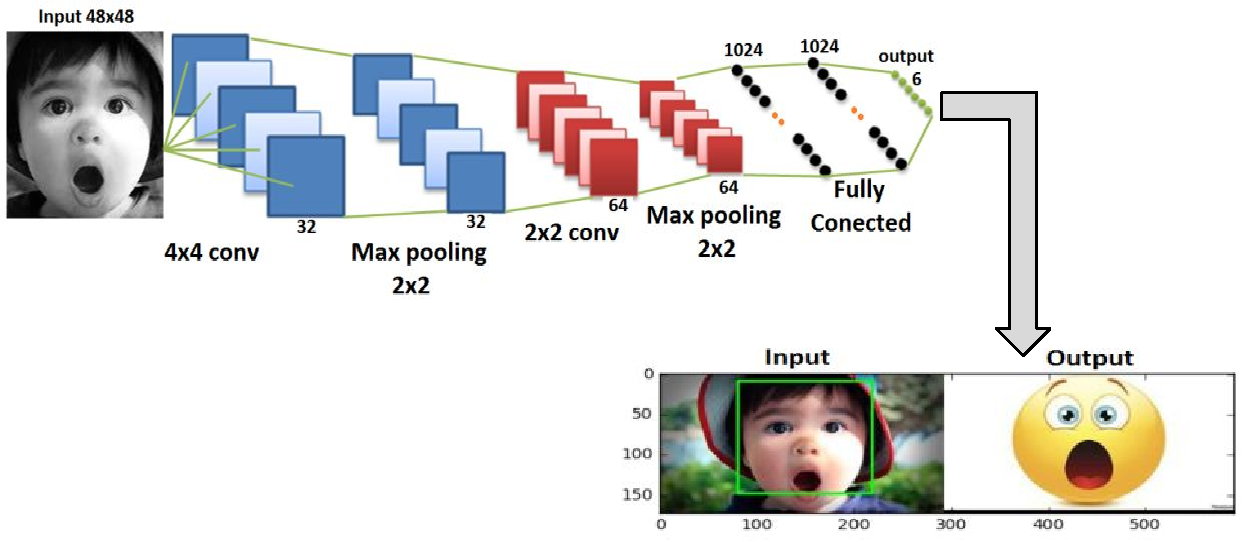
\includegraphics[width=180mm]{./Imagenes/arquitectura_CNN_grafico.pdf}
		\caption{Arquitectura grafica del modelo propuesto.}
		\vspace{0.15cm}
		\textit{Fuente: Propio.}
		\label{fig:arquitectura_CNN_grafico}
\end{figure}

La tabla~\ref{tab:tabla_arquitectura} muestra de arriba para abajo, la representación secuencial de las capas dentro de la arquitectura propuesta antes mencionada. Sin embargo, La figura~\ref{fig:arquitectura_CNN_grafico} muestra de una forma mas detallada cada una de las capas que integran la arquitectura, construyendo de esta forma una red neuronal convolucional. Tambien se muestra en esta figura, la salida final obtenida despues de realizar una consulta sobre el modelo, resaltando el rostro detectado en la imagen de entrada, y relacionando la expresion facial que este tiene con una imagen caricaturizada.

\section{Descripción de la Capas de la Arquitectura}

Dentro de cada capa perteneciente a la red neuronal convolucional, se lleva a cabo operaciones de multiplicacion de matrices, agrupacion de regiones, etc, con el objetivo de extraer o resaltar características importantes de las cuales la red pueda aprender patrones y filtros que se adanten mejor al problema, de tal forma que pueda dar respuestas precisas a entradas futuras. 

Siguiendo el orden de capas de la arquitectura propuestas, presentada en la seccion~\ref{sec:arq_propuesta}, se describe el comportamiento de cada uno de ellos de la siguiente forma: 
\begin{itemize}
\item
{
\textbf{Primera capa convolución.} Cuenta con 32 filtros (mapa de características) de tamaño 4x4 pixeles. Esta capa tiene como objetivo extraer características de alto nivel. La figura~\ref{fig:filtro1} muestra el conjunto de imagenes generadas despues de aplicar los 32 filtros de convolución sobre la imagen de entrada, estas imagenes muestra claramente que en esta capa, la arquitectura se encarga de aprender filtros que sean capaces de extraer bordes y partes fundamentales del rostro, tales como: los ojos, boca, nariz y cejas. Esta primera capa de convolución genera una imagen de salida por cada filtro, siendo así, 32 nuevas imágenes las entradas para la siguiente capa. 

\begin{figure}[H]
		\centering
		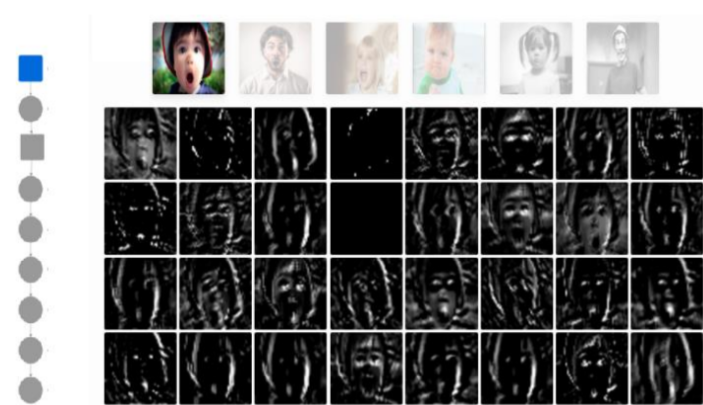
\includegraphics[width=100mm]{./Imagenes/filtro1.png}
		\caption{Imágenes de salida después de la primera convolución.}
		\vspace{0.15cm}
		\textit{Fuente: Propio.}
		\label{fig:filtro1}
\end{figure}
}

\item
{
\textbf{Primera capa de \textit{pooling} o sub-muestreo.} Recibe como parámetros de entrada, las 32 imágenes generadas a partir de la primera capa de convolución. Su función es la de reducir características redundantes mediante la agrupación de pixeles y eleccion del mejor de entre ellos, esta agrupacion se realiza en sub-regiones no solapadas de la matriz, de dimensiones 2$\times$2. Despues de obtener estas sub-regiones, se obtiene el maximo pixel de entre ellas para ser la salida de dicha sub-region. La figura~\ref{fig:filtro2} muestra imágenes semejantes a las obtenidas por la primera capa de convolución, esto se debe a que esta capa no realiza ninguna alteración en el valor de los píxeles, mas al contrario, esta encargada de reducir las dimensiones de las imágenes de entrada, eliminando los píxeles menos significativos. Debido a que se aplica este tipo de operaciones a cada imagen de entrada de esta capa, su número de imágenes de salida sera igual a su numero de entradas.

\begin{figure}[H]
		\centering
		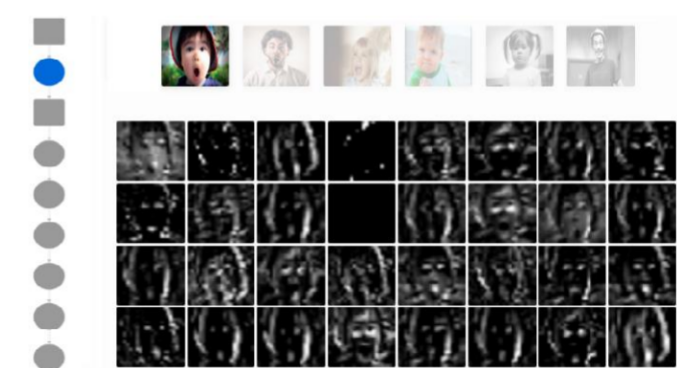
\includegraphics[width=100mm]{./Imagenes/filtro2.png}
		\caption{Imágenes de salida después del primer sub-muestreo.}
		\vspace{0.15cm}
		\textit{Fuente: Propio.}
		\label{fig:filtro2}
\end{figure}
}

\item
{
\textbf{Segunda capa de convolución.} Cuenta con 64 filtros y recibe como parámetros de entrada las imágenes generadas a partir de la primera capa de sub-muestreo. A diferencia de la primera capa de convolución, su funcion es la de extraer y detectar caracteristicas de mas bajo nivel. La figura~\ref{fig:filtro3} muestra las 64 imagenes generadas a partir los filtros de esta capa, en ellas se puede observar de manera mas abstracta ciertos puntos y rectas que representan partes del rostro de la imagen de entrada. Como se menciono anteriormente, esta capa origina 64 imágenes de salida, cada una con un tamaño de 21$\times$21 píxeles.

\begin{figure}[H]
		\centering
		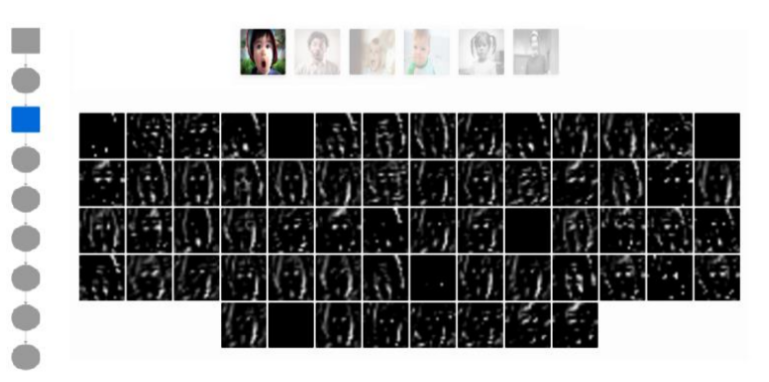
\includegraphics[width=100mm]{./Imagenes/filtro3.png}
		\caption{Imágenes de salida después de la segunda convolución.}
		\vspace{0.15cm}
		\textit{Fuente: Propio.}
		\label{fig:filtro3}
\end{figure}
}

\item
{
\textbf{Segunda capa de \textit{pooling} o sub-muestreo.} Recibe como parámetros de entrada las imágenes generadas a partir de la segunda capa de convolución. Similar que la primera capa de sub-muestreo, es la encargada de eliminar características no relevantes de las imágenes de entrada, mediante la agrupación y selección del mejor píxel, las sub-regiones de agrupacion son de dimensiones 2$\times$2. La figura~\ref{fig:filtro4} muestra las 64 imágenes generadas a partir de esta capa, donde cada una de estas nuevas imágenes son de tamaño 10x10 pixeles. Segun esta figura se puede observar que el rostro se distorsiona y pierde su forma original, siendo estas, a lo que se conoce como características de bajo nivel.
\begin{figure}[H]
		\centering
		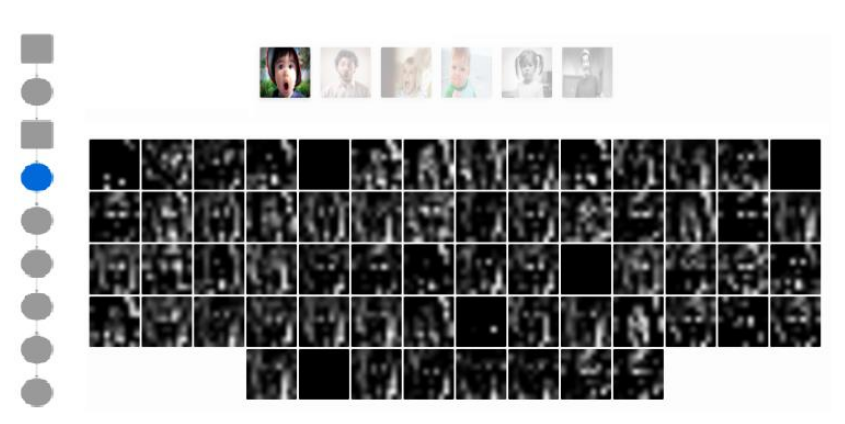
\includegraphics[width=100mm]{./Imagenes/filtro4.png}
		\caption{Imágenes de salida después del segundo sub-muestreo.}
		\vspace{0.15cm}
		\textit{Fuente: Propio.}
		\label{fig:filtro4}
\end{figure}
}
\item
{
\textbf{Capas totalmente conectadas.} Recibe como parámetros de entrada las imágenes generadas a partir de la segunda capa de sub-muestreo, las cuales representan las caracteristicas a bajo nivel pertenecientes a la imagen de entrada original. El objetivo de esta capa, es relacionar cada una de estas características por medio de las 2 capas totalmente conectadas con 1024 neuronas cada una, donde cada neurona es una imagen que representa alguna caracteristica encontrada en las capas anteriores. Al final de la arquitectura, se utiliza la función de normalización \textit{softmax} para generar 6 salidas, donde cada una de ellas representa a una expresion facial. La funcion de normalizacion es la encargada de asignar una probabilidad a cada una de estas salidas, siendo nuestra salida final, aquella que presente la mayor probabilidad.
}
\end{itemize}

\section{PARAMETROS DE LA ARQUITECTURA}
La imágenes de entrada son definidas en el tamaño de 48x48 píxeles como valor
estándar basándonos en el tamaño en el cual están las imágenes de la base de datos
FER2013, el número de convoluciones en la primera capa es de 32 y 64 en la segunda
capa de convolución obteniendo así un total de 32x64 mapas de características, la capa
de Pooling agrupa subregiones de las dimensiones 2x2 píxeles para que no se pierda
mucha información, nosotros optamos por la elección de dos capas totalmente conectadas
de 1024x1024 producto de los resultados obtenidos basándonos en prueba y error , el total
de parámetros obtenidos con la arquitectura propuesta es de:

\begin{itemize}
\item Imagen de entrada: 48x48 píxeles
\item 1ra capa con 32 convoluciones: 544 parámetros
\item 2da capa con 64 convoluciones: 8256 parámetros
\item 1ra capa totalmente conectada: 6554624 parámetros
\item 2da capa totalmente conectada: 1049600 parámetros
\item función de normalización Softmax: 7175 parámetros
\end{itemize}
Obteniendo un total de 7,620,199 parámetros totales.

\begin{table}[H]
    \centering
    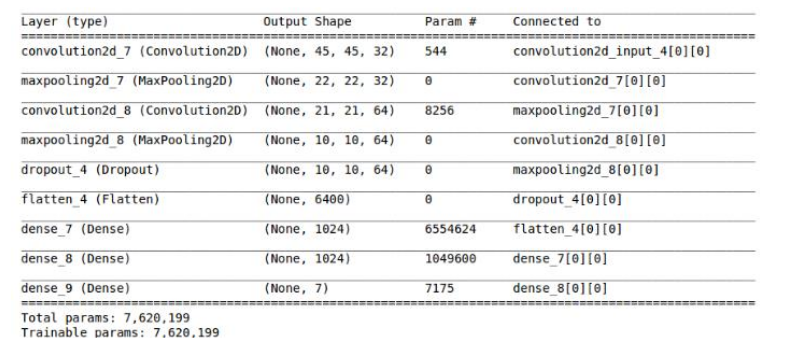
\includegraphics[width=140mm]{./Imagenes/parametros.png} 
    \caption{Número de parámetros de nuestra CNN}
    \label{tab:parametros}
\end{table}

	
\section{ENTRENAMIENDO DE LA CNN}
El entrenamiento de nuestra Red Neuronal Convolucional siguió un proceso
iterativo en el que se presentó como datos de entrada imágenes de expresiones faciales y
sus respectivas etiquetas de salida (clases correspondientes a la expresión facial a la cual
pertenece: enojo, miedo, alegría, tristeza, sorpresa y neutro).

Durante esta fase de entrenamiento, la Red Neuronal Convolucional aprendió
mediante el ajuste de sus pesos, con el fin de ser capaz de predecir la etiqueta de clase
correcta de los datos de entrada, el algoritmo de Red Neuronal más popular para la fase
de entrenamiento es el algoritmo de BackPropagation, dicho algoritmo se usó en nuestra
fase de entrenamiento. Los pesos iniciales de nuestra red se eligieron al azar y comienza
el entrenamiento o aprendizaje. Se procesó los datos de entrada para lograr obtener las
etiquetas deseadas obteniendo un error el cual se propago hacia atrás mediante el
algoritmo antes mencionado(BackPropagation) haciendo que se ajusten los pesos, este
proceso ocurrió una y otra vez hasta que se minimizo el error y eso ocurrió cuando se
logró una convergencia de los datos.

\section{TEST AL MODELO CREADO}
Una vez creada el modelo (un archivo con extensión .h5) se procede a realizar las
consultas a dicho modelo, estas consultas siguen los siguientes pasos:

\begin{itemize}
\item Leer una imagen de entrada, de dimensiones mayos o igual a 48x48 pixeles.
\item Utilizar Haar Cascade para la detección del rostro en la imagen antes ingresado.
\item Extraer el rostro detectado y redimensionarlo al tamaño 48x48 pixeles.
\item Dar como imagen de entrada la imagen obtenida en el paso anterior.
\end{itemize}
Después de realizar los pasos anteriores, el modelo arrojara un valor asociado a la
expresión facial predicha.

\section{RECOPILACIÓN DE IMAGENES DE EXPRESIONES
FACIALES}
La recopilación de las imágenes de expresiones faciales se obtuvo de 2 fuentes
secundarias de información (internet) en los cuales los datos están pre-elaborados
(imágenes con tamaños de 48x48 pixeles de base de datos FER20131 y 640x490 o
640x480 píxeles de la base de datos CK+).

\section{BASE DE DATOS}
Se usó 3 bases de datos ($FER2013^{1}$ y $CK+^{2}$ ) y una tercera como resultado de la
unión de las 2 bases de datos antes mencionadas.
\subsection{FER2013}
Es una base de datos del sitio web Kaggle{1} para el concurso de reconocimiento de
expresiones faciales.

Esta base de datos posee 35887 imágenes en escala de gris de 48x48 pixeles,
clasificados en 7 categorías (enojado, disgustado, miedo, feliz, triste, sorpresa y neutro).
En este trabajo se optó por unir la categoría enojado y disgustado por las similitudes que
tienen entre ellas.

Separamos la data en 2 partes training y test. El training consta de 32298 imágenes
y el test de 3589 imágenes.

\begin{figure}[H]
		\centering
		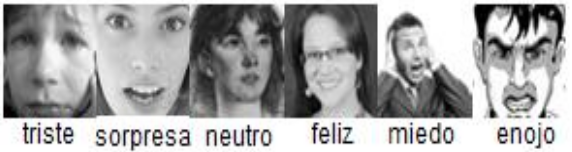
\includegraphics[width=90mm]{./Imagenes/imagenes_fer.png}
		\caption{Imágenes de la base de datos FER2013}
		Source: Kaggle
		\label{fig:imagenes_fer}
\end{figure}

\section{CK+}
La base de datos $CK+^{2}$ (Cohn-Kanade) posee imágenes de expresiones faciales
frontales de 210 personas en resolución de 640x490 o 640x480 pixeles. Nosotros
elegimos de entre ellos 3289 imágenes convirtiéndolos a escala de gris de 48x48 pixeles
y clasificándolos en 6 categorías (enojado, miedo, feliz, triste, sorprendido y neutro).
Nuestro training consta de 2966 imágenes y el test de 323 imágenes.

\begin{figure}[H]
		\centering
		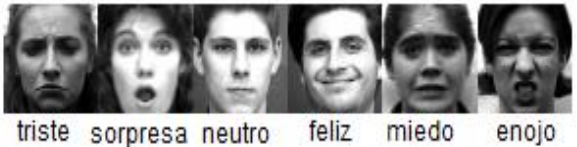
\includegraphics[width=90mm]{./Imagenes/imagenes_ck+.png}
		\caption{Imágenes de la base de datos CK+}
		Source: Base de datos CK+
		\label{fig:imagenes_ck+}
\end{figure}


\section{FER2013 - CK+}
Esta base de datos resulta de la unión de la base de datos Fer2013 y CK+,
obteniendo un total de 39176 imágenes de 48x48 en escala de gris. El training tiene 35264
y el test 3912 imágenes.

\section{RESULTADOS EXPERIMENTALES}
A continuación, se muestra los resultados que se obtuvieron en las diferentes bases
de datos FER2013, CK+ y la tercera base de datos que se obtuvo como resultado de la
unión de los dos antes mencionadas.

Se podrá apreciar los niveles de precisión alcanzado por cada categoría –
Expresión Facial (Enojado, Miedo, Feliz, Triste, Sorprendido, Neutro). Así como sus
matrices de confusión que nos mostraran los resultados positivos y sus falsos positivos,
pudiendo así interpretar de mejor manera los resultados.

\subsection{FER2013}

\begin{table}[H]
    \centering
    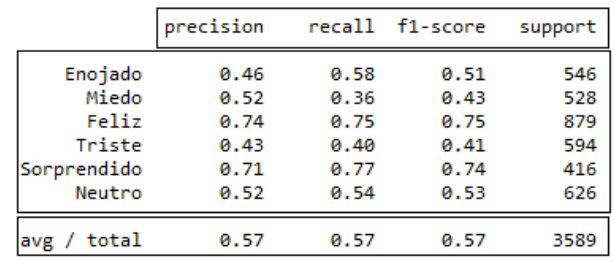
\includegraphics[width=80mm]{./Imagenes/tabla_resultados_fer.png} 
    \caption{Resultados obtenidos - FER2013}
    \label{tab:tabla_resultados_fer}
\end{table}

En la Tabla 3 se puede apreciar los niveles de precisión en la clasificación de los
datos de la base de datos FER2013, mostrando en la categoría Enojado 46\%, Miedo 52\%,
Feliz 74\% Triste 43\%, Sorprendido 71\% y Neutro 52\%.

\begin{figure}[H]
		\centering
		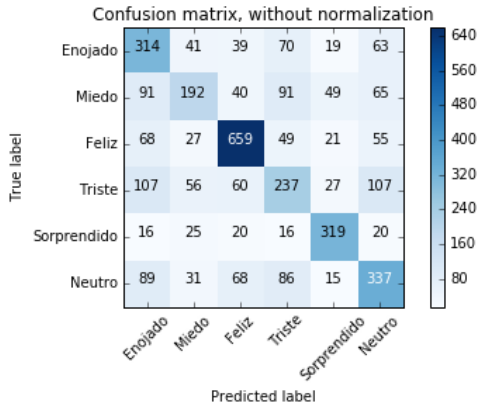
\includegraphics[width=80mm]{./Imagenes/matriz_confusion_fer.png}
		\caption{Matriz de confusión, precisión del Test - FER2013}
		\label{fig:matriz_confusion_fer}
\end{figure}

\begin{figure}[H]
		\centering
		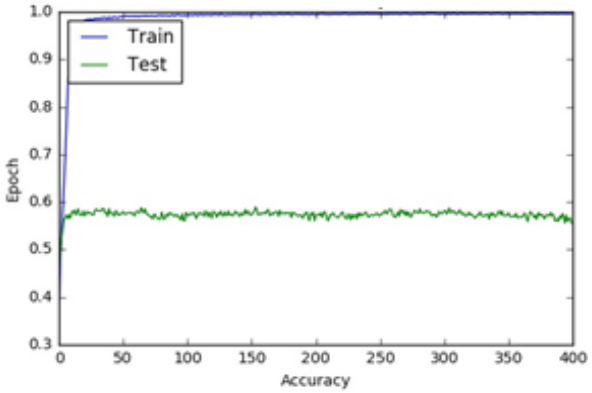
\includegraphics[width=80mm]{./Imagenes/precision_fer.png}
		\caption{Precisión durante el proceso de entrenamiento y prueba (\%) – FER2013}
		\label{fig:precision_fer}
\end{figure}

\begin{figure}[H]
		\centering
		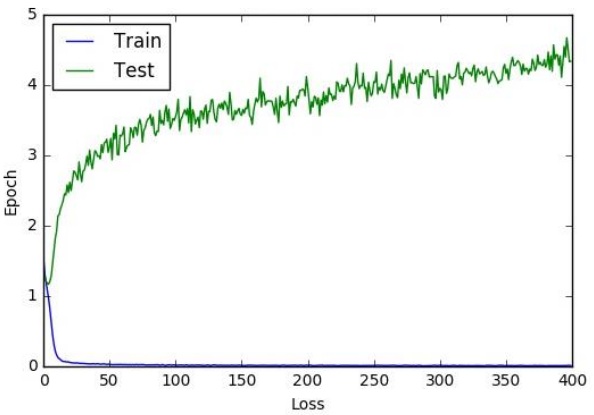
\includegraphics[width=80mm]{./Imagenes/perdida_fer.png}
		\caption{Perdida durante el proceso de entrenamiento y prueba (\%) – FER2013}
		\label{fig:perdida_fer}
\end{figure}

\subsection{CK+}

\begin{table}[H]
    \centering
    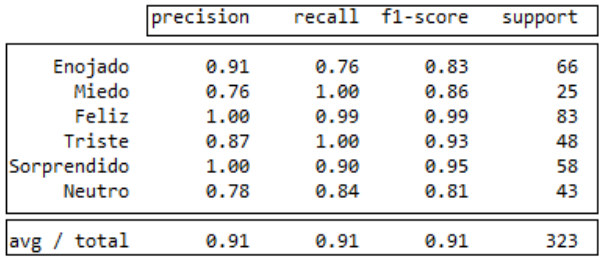
\includegraphics[width=80mm]{./Imagenes/tabla_resultados_ck+.png} 
    \caption{Resultados obtenidos - CK+}
    \label{tab:tabla_resultados_ck+}
\end{table}

En la Tabla 4 se puede apreciar los niveles de precisión en la clasificación de los
datos de la base de datos CK+, mostrando en la categoría Enojado 91\%, Miedo 76\%,
Feliz 100\%, Triste 87\%, Sorprendido 100\% y Neutro 78\%.

\begin{figure}[H]
		\centering
		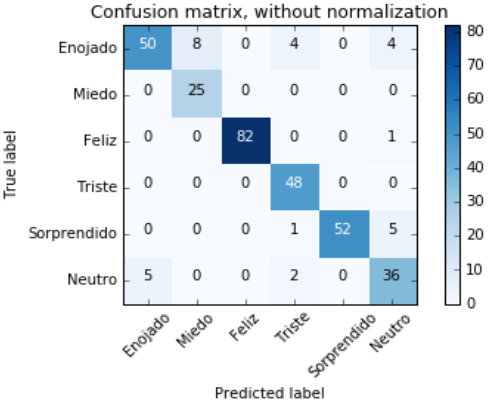
\includegraphics[width=80mm]{./Imagenes/matriz_confusion_ck+.png}
		\caption{Matriz de confusión, precisión del Test - CK+}
		\label{fig:matriz_confusion_ck+}
\end{figure}

\begin{figure}[H]
		\centering
		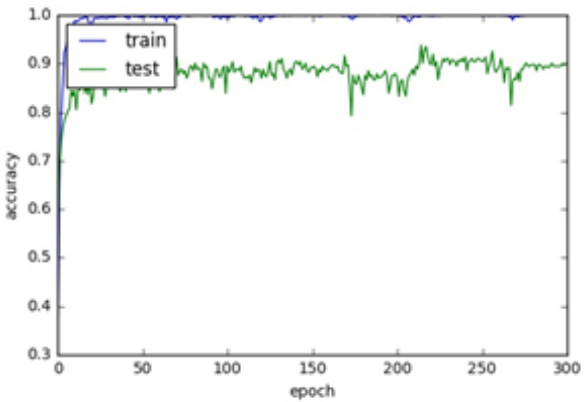
\includegraphics[width=80mm]{./Imagenes/precision_ck+.png}
		\caption{Precisión durante el proceso de entrenamiento y prueba (\%) - CK+}
		\label{fig:precision-ck+}
\end{figure}

\begin{figure}[H]
		\centering
		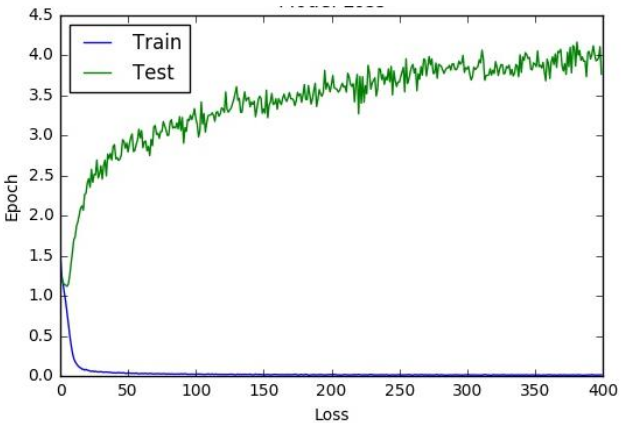
\includegraphics[width=80mm]{./Imagenes/perdida_ck+.png}
		\caption{Perdida durante el proceso de entrenamiento y prueba (\%) – FER2013}
		\label{fig:perdida_ck+}
\end{figure}

\subsection{FER2013 - CK+}


\begin{table}[H]
    \centering
    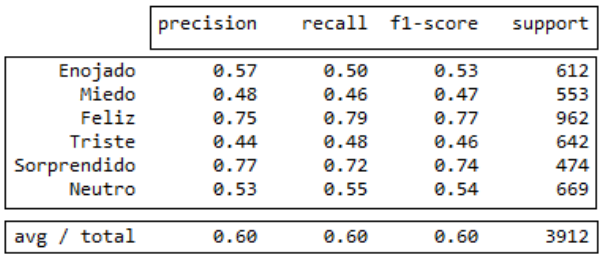
\includegraphics[width=80mm]{./Imagenes/tabla_resultados_fer_ck+.png} 
    \caption{Resultados obtenidos - FER2013 - CK+}
    \label{tab:tabla_resultados_fer_ck+}
\end{table}

En la Tabla 5 se puede apreciar los niveles de precisión en la clasificación de los
datos de la base de datos (FER2013 - CK+), mostrando en la categoría Enojado 57\%,
Miedo 48\%, Feliz 75\%, Triste 44\%, Sorprendido 77\% y Neutro 53\%

\begin{figure}[H]
		\centering
		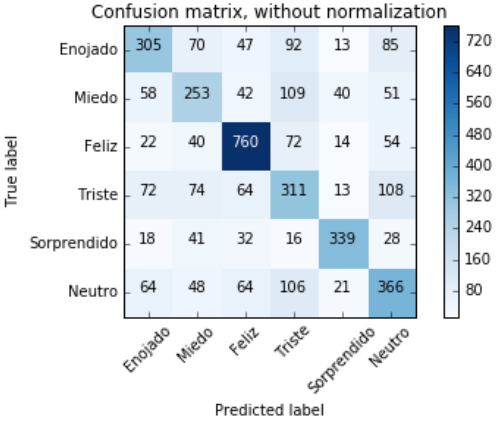
\includegraphics[width=80mm]{./Imagenes/matriz_confusion_fer_ck+.png}
		\caption{Matriz de confusión, precisión del Test FER2013 - CK+}
		\label{fig:matriz_confusion_fer_ck+}
\end{figure}

\begin{figure}[H]
		\centering
		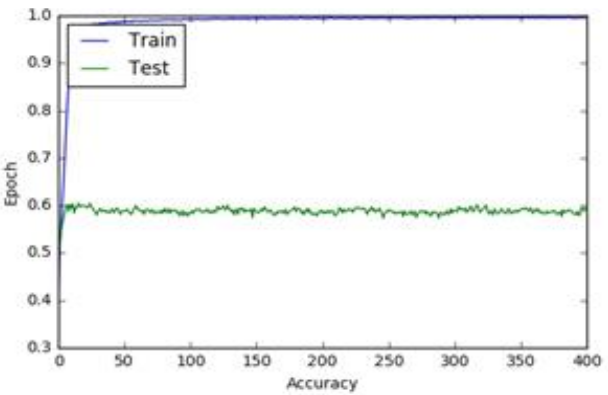
\includegraphics[width=80mm]{./Imagenes/precision_fer_ck+.png}
		\caption{Precisión durante el proceso de entrenamiento y prueba (\%) FER2013 - CK+}
		\label{fig:precision_fer_ck+}
\end{figure}

\begin{figure}[H]
		\centering
		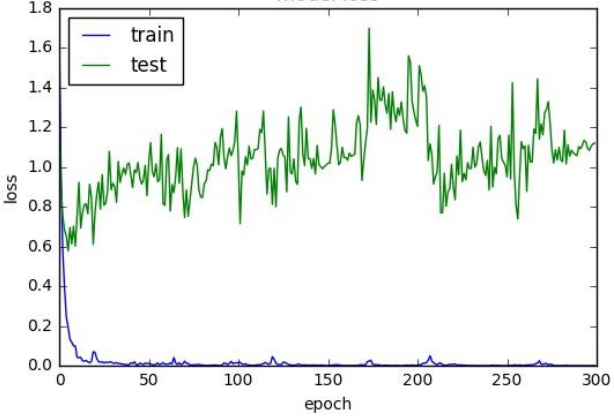
\includegraphics[width=80mm]{./Imagenes/perdida_fer_ck+.png}
		\caption{Perdida durante el proceso de entrenamiento y prueba (\%) FER2013 - CK+}
		\label{fig:perdida_fer_ck+}
\end{figure}


